\documentclass[a4paper,10pt]{article}
\usepackage[hidelinks]{hyperref}
\def\UrlBreaks{\do\/\do-} % breaks long url in references
\usepackage{graphicx}
\usepackage[english]{babel}
\usepackage{listings}
\usepackage[labelfont=it,textfont={it},singlelinecheck=on,justification=centering]{caption}
\usepackage{amsmath}
\usepackage{float}
\usepackage{draftwatermark}
\SetWatermarkLightness{0.97}
\DeclareGraphicsExtensions{.pdf,.png,.jpg}
\begin{document}
\lstset{basicstyle=\ttfamily\footnotesize,breaklines=true}
\lstset{numbers=left, numberstyle=\tiny, stepnumber=1, numbersep=5pt}
\lstset{language=TeX}
\SetWatermarkScale{8}

\title{\large \bf Storj:  Peer-to-Peer Cloud Storage Network}
\author{\small Shawn Wilkinson + Vitalik Buterin\\ \small shawn@storj.io + v@buterin.com \\ }
\maketitle
\begin{abstract}
A peer-to-peer cloud storage network implementing end-to-end encryption would allow users to transfer and share data without reliance on a third party data provider. The removal of central controls would eliminate the possibility of traditional data failures and outages, as well as significantly increase security and privacy. A peer-to-peer network and basic encryption serve as a solution for most problems, but is not useful if the network can be subjected to Sybil attacks or suffer from file losses from peer disconnects. We propose a solution to these additional problems by using a hash challenge algorithm. Redundant copies are uniquely encrypted, and the hosting node must hash the data and a given seed to return a unique hash. These unique hashes not only serve as proof that the file is being stored, but also that it remains unmodified. Furthermore, failure of these challenges will initiate a process to restore the desired redundancy. In this way, a single honest node can verify the integrity and availability of the file, and malicious nodes will not be able to complete challenges and are thus dropped from the network. 
\end{abstract}

\section{Introduction}
Cloud storage on the Internet has come to rely almost exclusively on data providers serving as trusted third parties to transfer and store the data. While the system works well enough in most cases, it still suffers from the inherent weaknesses of the trust-based model. Because end-to-end encryption is non-standard, the traditional cloud is open to a variety of security threats, including man-in-the-middle attacks, malware, and application hacks that expose sensitive and private consumer and company data. Furthermore, current cloud storage applications are able to charge large premiums on data storage over their core costs because users have few interoperable and featureful providers to choose from. Moreover, these third party providers may have technical failures that can cause data loss and unavailability, much to the distress of the users and applications that depend on them. These shortcomings were discussed in greater depth in our previous white paper \cite{1}.\\

What is needed is a decentralized cloud storage platform that implements end-to-end encryption on a decentralized and open network, instead of those hosted by third party data providers. This platform must be resistant to attackers who might attempt Sybil attacks and other forms of fraud. Furthermore, this network must account for the latency, performance, and downtime of an average consumer computer.\\

In our proposed network, cryptographic algorithms would protect data in transit and on devices not controlled by the user. An open market would eliminate the large premiums by allowing all data to be equally traded across the network. Because most internet-connected computers have unused hard drive space, users could sell these resources to the network. Periodic checks through hashing could verify the integrity and availability of a file on this network. \\

\section{Files as Encrypted Chunks}
We identify a chunk as an encrypted portion of a file that we would like to store on this network. Splitting the file into chunks allows for better data security so that no one farmer will have a complete copy as long as the file being stored is above a standardized chunk size. We define a farmer as a user that is leasing his or her hard drive space to the network. We define a standardized chunk size as a byte multiple such as 8 MB or 32 MB. Chunks are kept in standardized sizes to dissuade any attempt to determine what is being stored. Chunking also allows large files to be more manageable as they are distributed throughout the network.\\

We convergently encrypt chunks while also allowing users to optionally add salt, so that we can enable strong deduplication on the network while still offering the user the option of privacy if they so choose. Encryption is done on the client computer and it stores the hashes and decryption keys. The hash is used to lookup the file on the network, and the decryption key is used to transcribe the file back into plaintext.\\

For a public file, the client can simply use the standard convergent encryption, and share the hash and decryption keys with the relevant parties. For private files, the client should add salt, which will protect the client even if an eavesdropper is listening over the data line, and the eavesdropper knows exactly what file it is looking for. Thanks to these methods, we can choose to transmit the files to the network over either secured or unsecured data lines.

%insert Figure 1
\begin{figure}[h!]
\centering
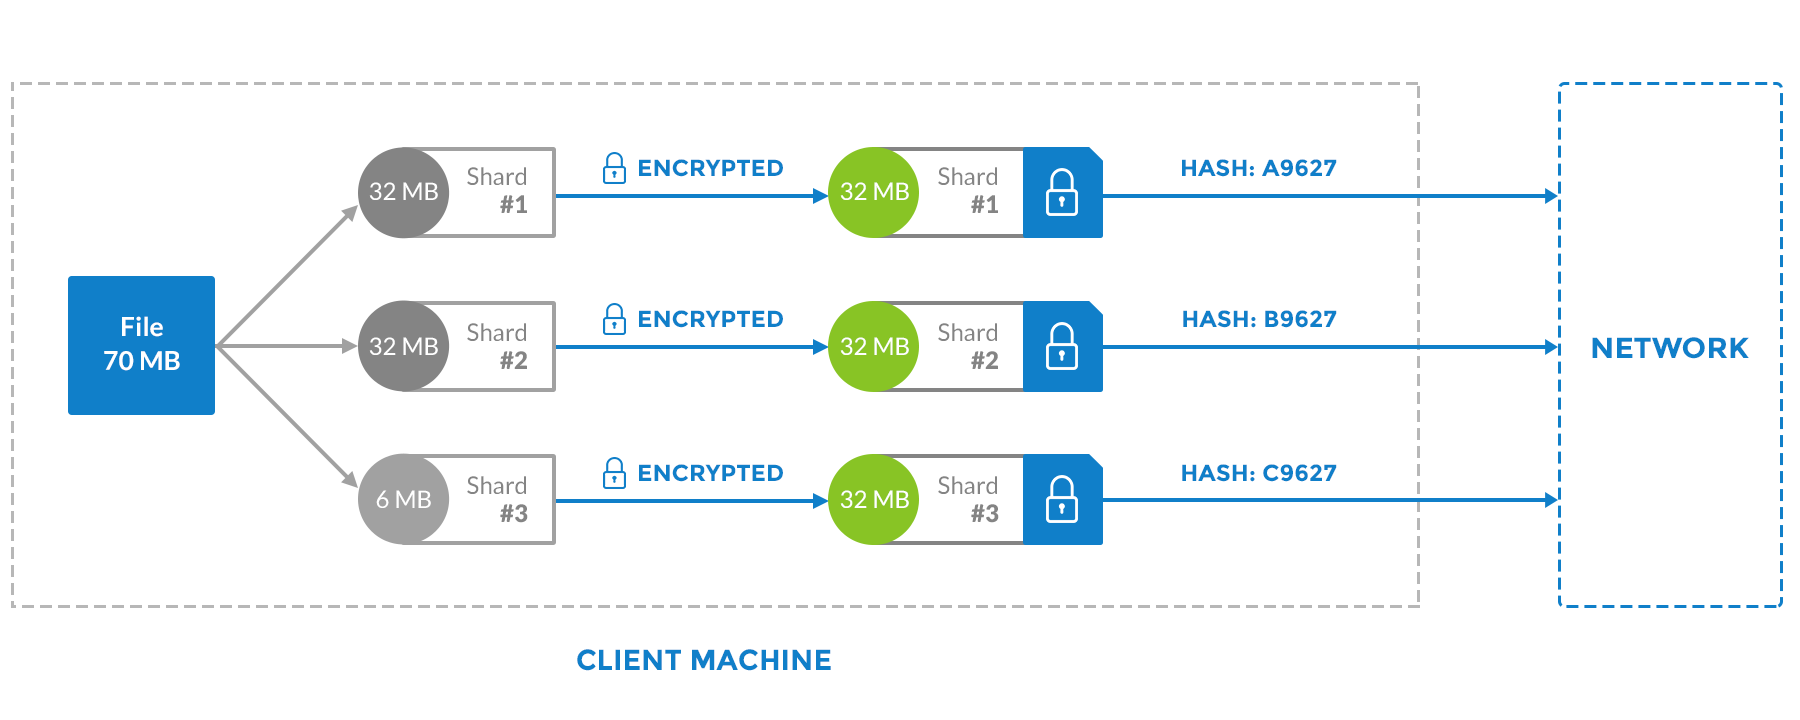
\includegraphics[width=\linewidth]{1}
\caption{Visualizing the Chunking Process}
\end{figure}

\section{Heartbeats}
To implement a trustless data storage network, we must provide a method for a client to verify that the data he or she has stored on the network is available and unmodified. We do this through a hash challenge, where the client creates a series of seeds (deterministically from a root seed) that can be added to the file and hashed to generate a unique hash answer. We refer to this process as a heartbeat. The client pre-generates these hash challenges, builds a Merkle tree \cite{2} and inserts the Merkle root into a Satoshi-style blockchain \cite{3}. The client can then periodically issue the seeds to farmers hosting its data, and check if that response matches its pre-generated hash answers.\\

The farmer cannot modify or delete the file because they will fail the hash challenges, as further described in “Proof-of-storage.”  By the premises of cryptography and hashing, these heartbeats cannot be brute forced. The client cannot cheat the farmer because the hash response can be verified via the Merkle root, which is inserted into a blockchain. In the case of a dispute, the client need only publish the Merkle tree, minus the leaves but including an extra hash, so that it can be verified. Challenges are issued to allow the farmer to also verify the integrity of the hash challenges as it completes them in groups of two (predicated on the publishing of the Merkle Tree minus the leaves) to the network. In this way we use blockchain backed proof-of-existence \cite{4} [5] to keep any party from acting maliciously.  \\

%insert Figure 2
\begin{figure}[h!]
\centering
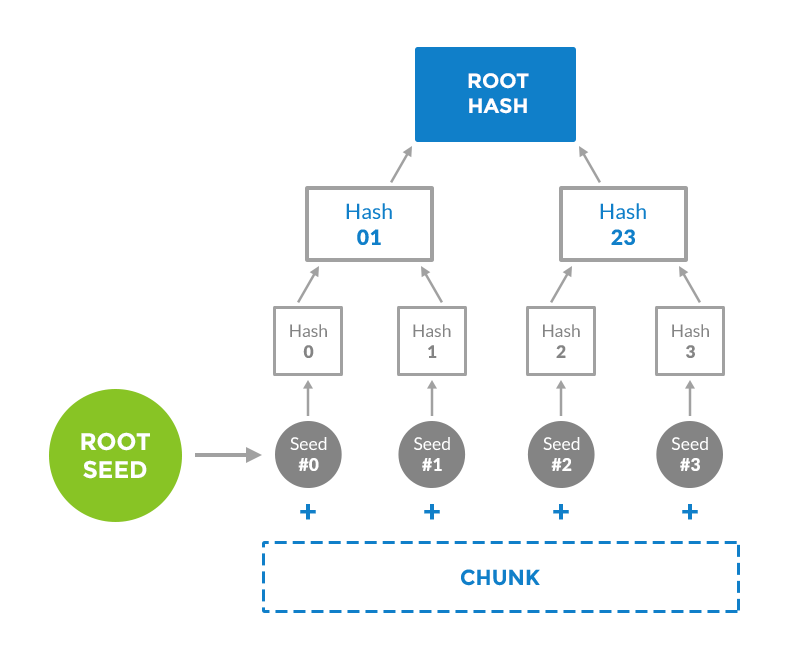
\includegraphics[width=\linewidth]{2}
\caption{Generating a Merkle Root for a Chunk}
\end{figure}


\section{Blockchain}
For the network to be able to achieve consensus on file location and integrity, we use Satoshi-style blockchains \cite{3}. As the blockchain is a public ledger, it is an excellent tool for retrieving accurate information, and as the ultimate mechanism to resolve disputes and dissuade attacks. To use a basic analogy, it is easy to steal a cookie from a cookie jar in a secluded area, but it is hard to do so when the jar is instead located in the middle of a public square being observed by thousands of people. By using a blockchain as a distributed data store, we can build off an established and time-tested distributed consensus mechanism. We do not store any files in the blockchain, but rather file metadata. In essence, we store the file hash, the network locations of the copies of the chunks, and Merkle roots of the heartbeats. The specifics and scalability of this method are described in the MetaDisk \cite{1} paper.  \\

%insert Figure 3
\begin{figure}[h!]
\centering
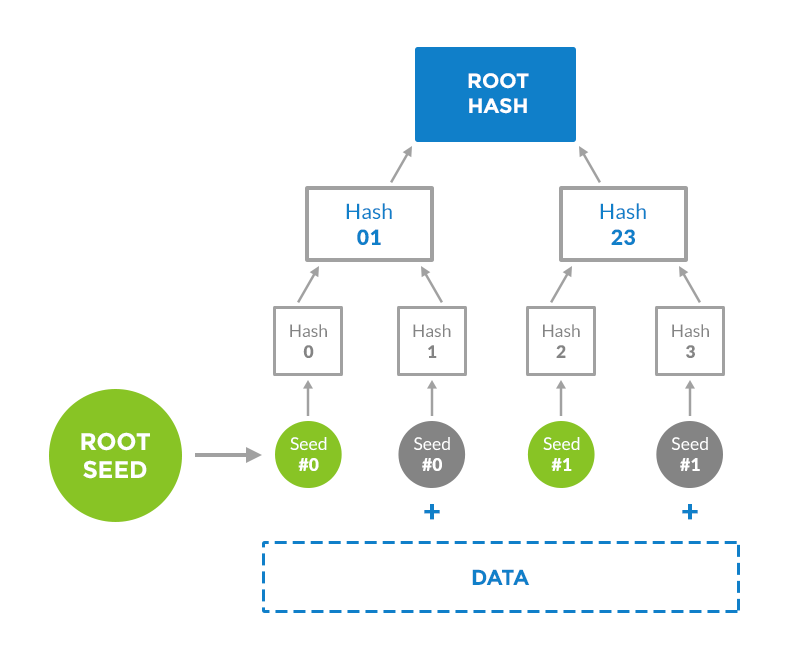
\includegraphics[width=\linewidth]{3}
\caption{Metadata Insertion into a Blockchain}
\end{figure}

Data is inserted into the blockchain via a standard transaction with extra metadata. Because this would be prohibitively expensive on the Bitcoin blockchain, and not technically feasible with the strict metadata limits on Bitcoin transactions, we do not use the Bitcoin blockchain to store this metadata. As described in the MetaDisk \cite{1} paper, we use Datacoin \cite{6} as an initial mechanism as we transition to a system where we use the Bitcoin blockchain more directly and in a more scalable manner, through proof-of-existence \cite{4} [5] \cite{7}.  

\section{Proof-of-Redundancy}
Traditional cloud storage companies own or lease servers to store their customers’ files. They use RAID schemes or a multi-datacenter approach to protect the file from physical or network failure. Storj has no physical servers - the files only exist on the distributed and decentralized network. Because of this, we must account for redundancy on the network rather than physically. We must also provide a solution to the predictable issue of farmers simply turning off their computers, removing the availability of a chunk from the network. \\

%insert Figure 4
\begin{figure}[h!]
\centering
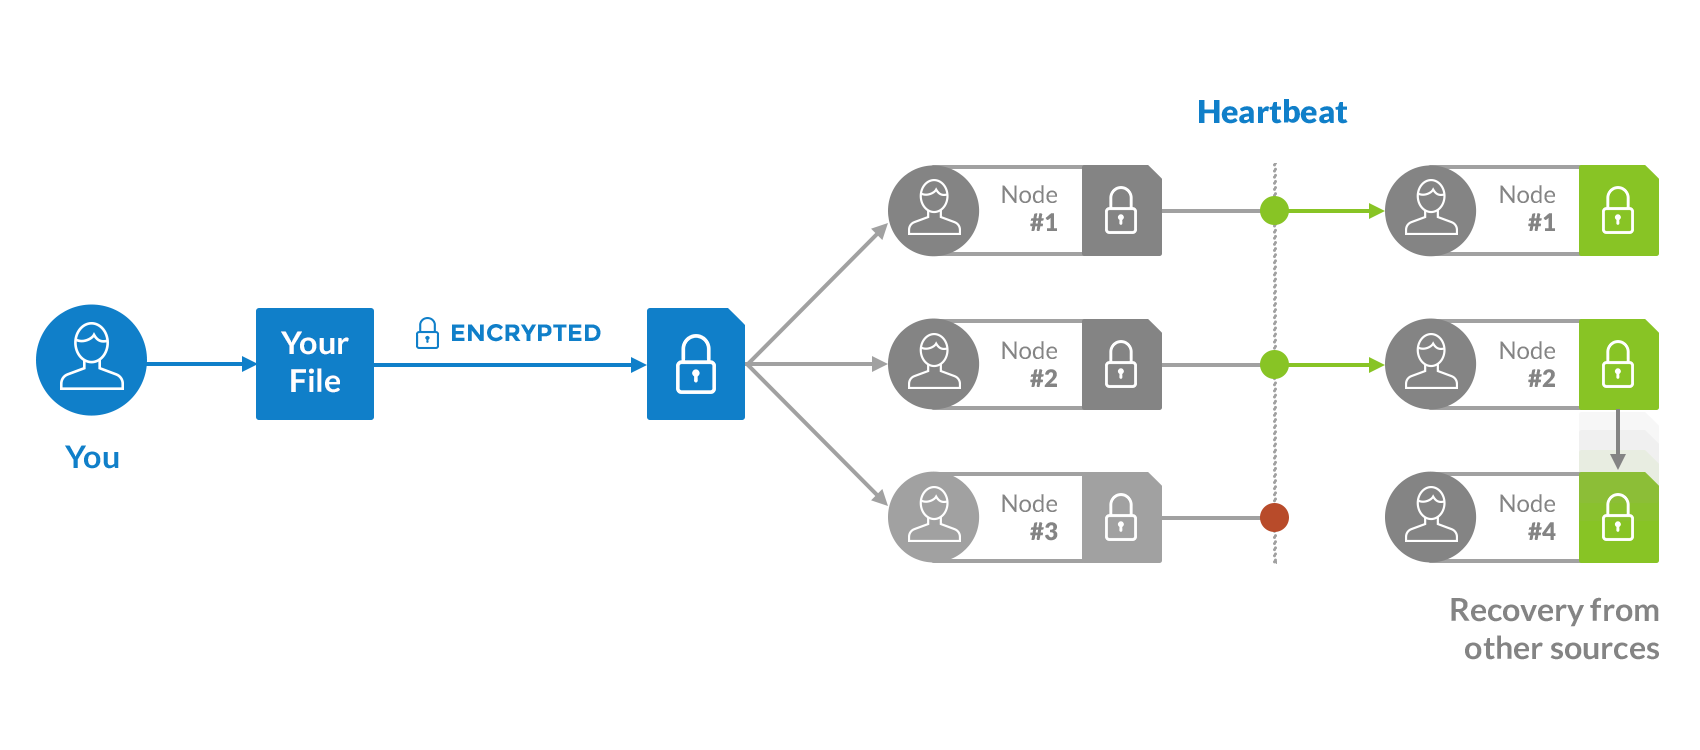
\includegraphics[width=\linewidth]{4}
\caption{Visualizing Heartbeats}
\end{figure}

If a node fails a heartbeat or is unreachable, we initiate a network replication process whereby we take one of the existing copies on network, and transfer it to another. The client must temporarily download the chunk to generate new challenges, or it can anticipate failure and pre-generate heartbeats based off of Node \#1 and Node \#2’s secondary copies. Because the chunk is already encrypted, we can use standard convergent encryption without any salt. Using headers we can specify how many layers of encryption there are to a particular chunk. \\

We must also address the problem of Sybil redundancy attacks. Because each redundant copy of a chunk is uniquely encrypted, malicious farmers can’t pretend to have multiple redundant copies of a file when they only have one. We can accomplish this by adding a deterministic salt value before convergently encrypting the chunk. We can base this value on our root seed. Even if the decryption key is known for a particular file, the malicious farmers will not be able to complete the hash challenges for copies they have not been assigned. In this way we can prove redundancy, because each redundant copy is unique.   \\

Through these methods, the network is able to heal itself based on periodic heartbeats. While we recommend the industry standard of 3x redundancy, the user or application can choose any redundancy \textit{r}. So, for a magnum opus, we might want to set a redundancy of 500x to protect the file against Armageddon and acts of God. As long as all \textit{r} nodes don’t disconnect from the network before the next heartbeat, the chunks are recoverable. 


\section{Speed}
Increased redundancy allows for some unique features on the Storj network. Because Storj is a decentralized and distributed network, upon addition of a new farmer to the network to host a chunk, we also add another peer that we can connect to download the chunk. If we set a redundancy of 20x, then we have 20 peers to download the chunk from simultaneously. This is in contrast the to the server-client model which relies on fast connections to the nearest data center.\\

%insert Figure 5
\begin{figure}[h!]
\centering
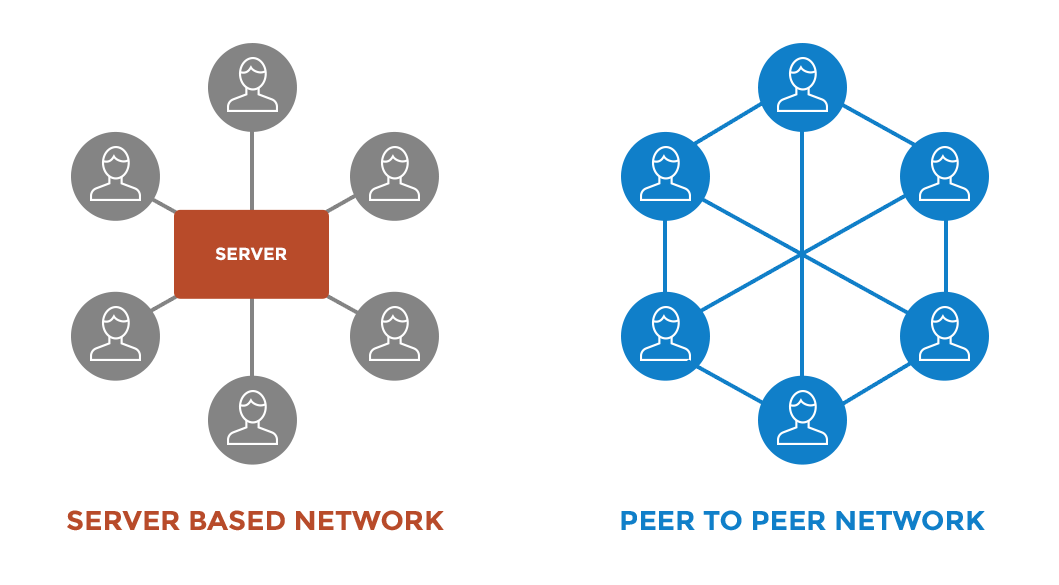
\includegraphics[width=\linewidth]{5}
\caption{Network Topology of a Server Based Network vs. a Peer to Peer Network}
\end{figure}

As with the standard functionality of a peer-to-peer network, we can connect to geographically close peers to achieve high transfer speeds. We can provide an incentive for peers to maintain node connectivity to the network using cryptocurrency, which solves the typical problem observed in peer-to-peer networks where there is insufficient peers for faster transfer. This concept is further described in the “Rewards” section. 

\section{Network Topology}
One of problems that we observed in the Bitcoin network was the declining number of full nodes on the network. “A healthy number of ‘full’ bitcoin nodes (those running the bitcoin core client on a machine instance with the complete block chain) are required to maintain and secure bitcoin’s distributed network. However, the total number of full nodes has declined in recent months and encouraging an uptake in node provisioning has proven difficult.” \cite{8} This is perhaps tied to to the fact that there is no inherent incentive in running a full node, which consumes large amounts of disk space and bandwidth. We instead pursued a model in which a full node on the network has a particular use case and adds value to the network. \\

%insert Figure 6
\begin{figure}[h!]
\centering
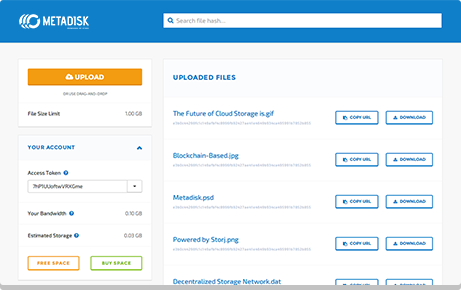
\includegraphics[width=\linewidth]{6}
\caption{Screenshot of the MetaDisk Application}
\end{figure}
We use our web application MetaDisk \cite{4} to function as a full node for the network. Users can optionally run the backend code for MetaDisk on their system to achieve the functionality of a full node. MetaDisk provides an interface for users and applications to interact with it, and it can optionally charge for the data services it provides. In this way, users have a direct incentive to run full nodes.  \\

%insert Figure 7 CITATION IN FIGURE TITLE!!!
\begin{figure}[h!]
\centering
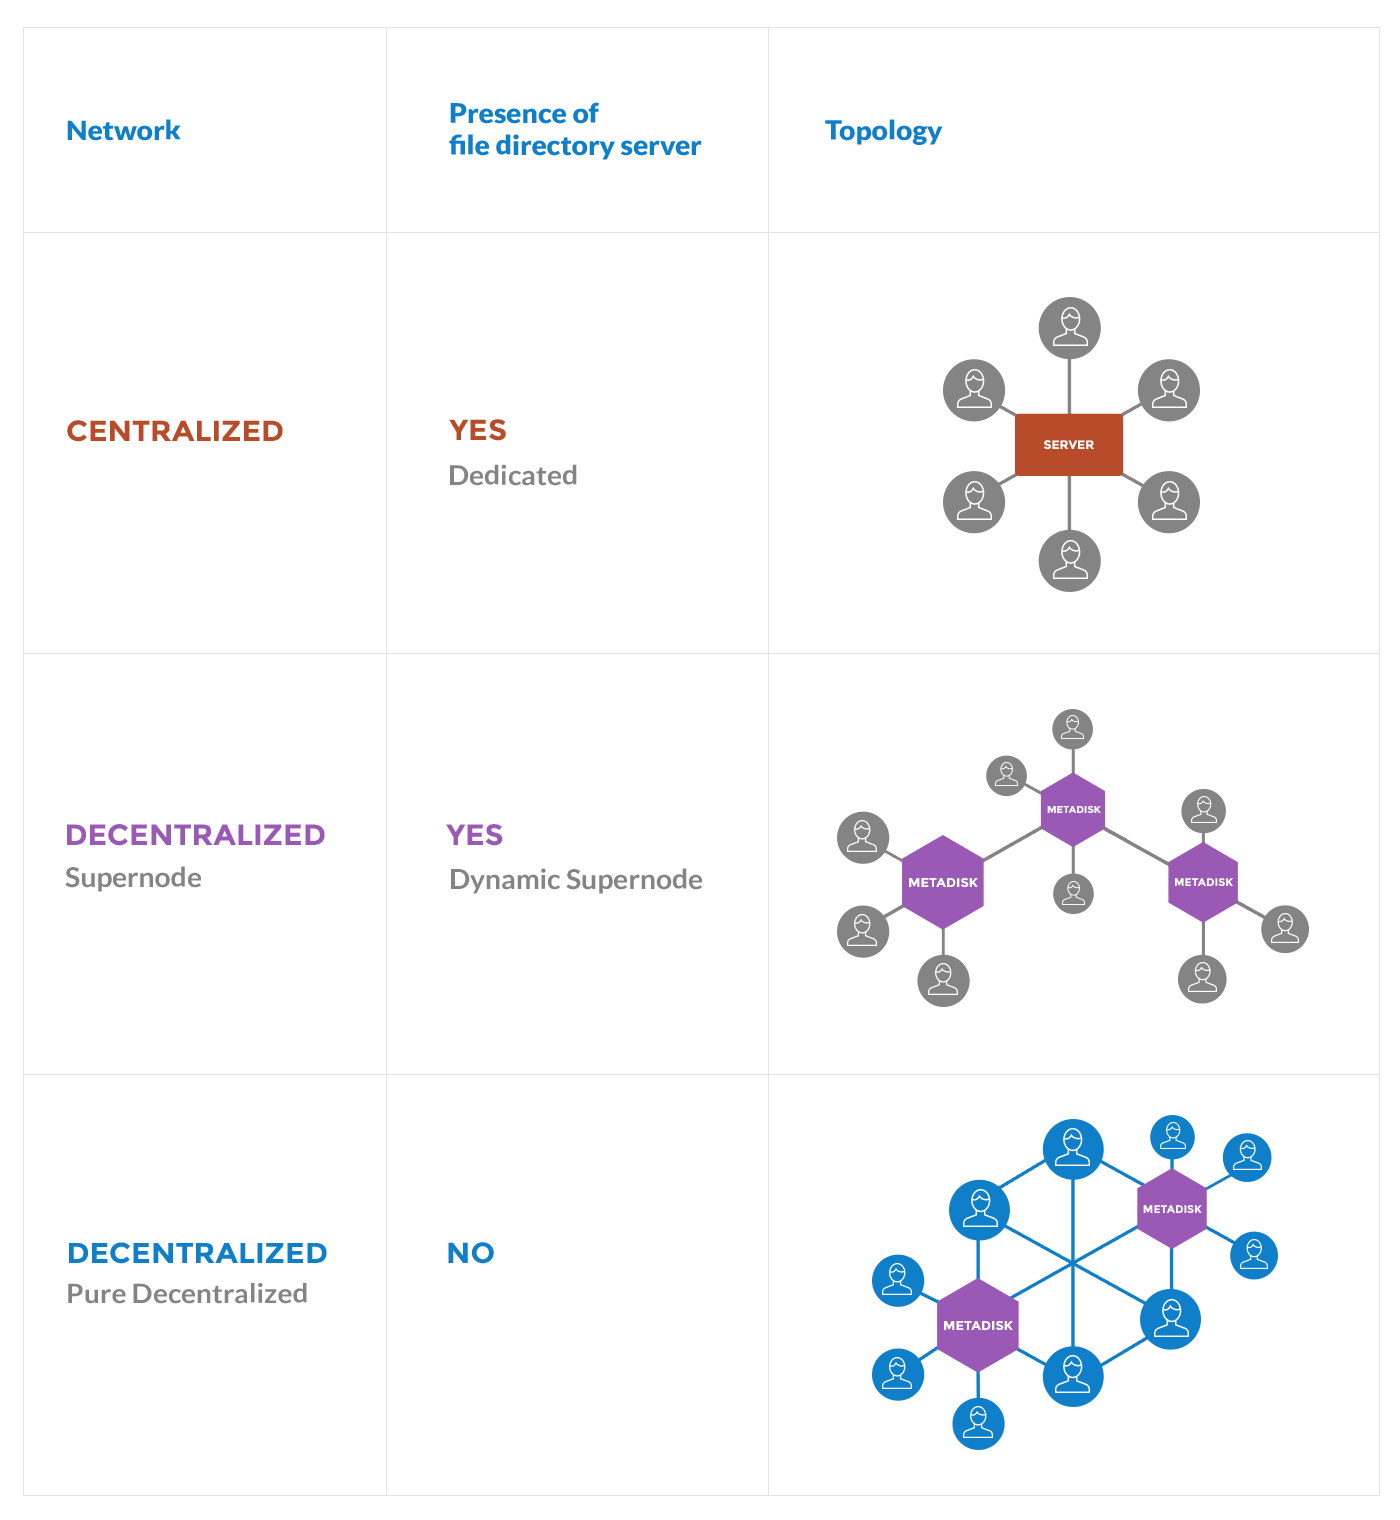
\includegraphics[width=\linewidth]{7}
\caption{Various Network Topologies \cite{9}}
\end{figure}
MetaDisk also helps bootstrap the early network by functioning as a supernode \cite{9}. During the early stages of the network, it can help with functions such as peer discovery. A client might want to store a file on the network with r=3. In this case, it needs to transfer its chunks to 3 locations, thus consuming bandwidth equivalent to 3x the file size. It instead can use a MetaDisk node to transfer the redundant copies to farmers, saving bandwidth on the client side. Farmers will always be looking for chunks to store, so they can also use MetaDisk nodes to find clients who need chunks stored, without having to traverse the peer-to-peer network.  \\

MetaDisk nodes can also help protect privacy. Even though files are encrypted, clients can instruct MetaDisk nodes to pass the file through other MetaDisk nodes before being stored, to mask the identity of the original client. This, combined with standardized chunking, and perhaps the addition of garbage chunks, traffic analysis of MetaDisk nodes, clients, and farmers—yield no useful information. Furthermore, just as Bitcoin mixing is implemented for increased privacy and security \cite{10}, data mixing can be implemented on the Storj network as a service with similar objectives. \\

As better peer-to-peer networking protocols and methods are established, the direct usefulness of MetaDisk nodes in the network will decrease. As it is a web application, it will transition to more of a Storj gateway, allowing more traditional services to interface with its API. This will allow users and applications to use the Storj network without installing additional software. We believe that abstraction and ease of use for end users and developers, rather than technical complexity, is the best way to help the Storj platform grow. \\

\section{Proof-of-Storage}
Another concern is the integrity and availability of a chunk stored on the network. A farmer must be able to prove cryptographically that it has the chunk, and has not modified it in any way. As described above, we use a heartbeat to accomplish this. More specifically, we generate hash challenges using 3 different methods.  \\

%insert Figure 8
\begin{figure}[h!]
\centering
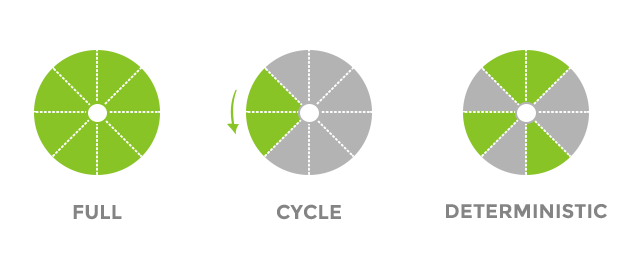
\includegraphics[width=\linewidth]{8}
\caption{Three Methods of Generating Hash Challenges}
\end{figure}

\subsection{Full Heartbeat}
We can use our seed and the full chunk to generate our hash response. This verifies full chunk integrity, but is extremely I/O-inefficient, and leads to long seek times.
\subsection{Cycle Heartbeat}
A small improvement is where the chunk is split into n discrete pieces, and we verify each piece in order until we complete the cycle. This method was first described in part by Filecoin \cite{11}. This is more I/O-efficient, and allows us to fully verify chunk integrity after n heartbeats. Unfortunately, it leaves the system open to potential attacks, as an attacker would still be able to complete heartbeats, with only a data integrity of 1/n.
\subsection{Deterministic Heartbeat}
In this method, we deterministically generate reads on a chunk using a root seed passed to us by the client. Because we cannot verify full integrity after n challenges, we add erasure encoding to our heartbeat scheme so that any minor changes to the chunk will be detected by the heartbeat, or recovered upon chunk retrieval. This is the most efficient method, and by adjusting our parameters we can balance I/O efficiency and file integrity verification.  
\subsection{Mixed Methodology}
Each method has its own advantages and disadvantages. We propose using a combination of these methods. It is recommended that a full heartbeat is used when the file is first uploaded to the network. Cycle heartbeats should be used periodically over some timescale. Deterministic heartbeats should be used for all other challenges. In this way, we can benefit from all the advantages offered by each algorithm. 


\section{Rewards}
For the network to function properly we must reward the correct and agreed upon behaviors. We use the cryptocurrency Storjcoin X, or SJCX, as the baseline currency for the Storj network. Clients and farmers can exchange SJCX for bandwidth and storage space on the network.\\

We can use micropayments/microtransactions \cite{12} \cite{13} to facilitate the instant transfer of cryptocurrency between nodes as payment for bandwidth or storage space. The client pays the farmer after the completion of a heartbeat. If both behave honestly and in agreement, no further steps are necessary. If not, the transaction will end and the last amount agreed upon will be considered final. We can alternately use trustless and automated mechanisms to perform disputes between nodes. As long as both parties are acting in a financially rational manner, these methods may not be necessary as the potential lost would only amount to a fraction of a cent. In the case of a targeted attack, where the attacker is only concerned with attacking the network at great financial expense, further mechanisms will be needed to protect new nodes on the network. 

\subsection{Market Basis}
Unlike traditional cloud services that implement fixed based pricing, pricing on the Storj network is determined by the market. The efficient allocation of data resources is enabled and incentivized by the free market. Farmers are able to set asks, and clients bids. Prices can vary based on bandwidth, location, and speed. For example, a fast server with SSD drives might charge more than a standard home laptop. In this way, we can achieve efficient usage of our data sources. Bob might want to store a video file on the network for streaming. In this case, Bob might want to use the fast SSD server. Alice might only be using the Storj network for backup purposes. In this case, the standard home laptop would serve as a more efficient and cheaper option

\subsection{Market Scale}
The market will also help balance the supply and demand of the storage space on the network. If there is an increased demand on the network for storage space then the SJCX token will increase in value, providing an incentive for farmers to add more storage space to the network to meet the demand. Likewise, as demand decreases, the storage price diminishes, slowing the growth of storage on the network. The network thus relies on the power of the market to ensure sufficient network resources 

\subsection{Peer Rewarding}
One of the problems that exists in traditional peer-to-peer networks is insufficient peers. Peers are simply volunteers which help enable very fast transfer speeds for very popular files. By the same token, a lack of peers sharing less popular files often leads to painstakingly slow transfer speeds or, simply, practically non-existent availability. Our inherent reward mechanism, based on SJCX, solves that problem by paying peers for holding chunks. Using micropayments/microtransactions, we can also more directly reward peers for transferring chunks to nodes that request them. In this way, peers may voluntarily host popular chunks so that they may earn more SJCX. In a nutshell, this system enables trustless yet incentivized transfers without relying upon the technical overhead of a proof-of-bandwidth algorithm. However, a recent paper on TorPath \cite{14} has shed some light on how that might be possible.  

\subsection{Uptime}
Farmers are encouraged to have high uptime. This could be quite easy for dedicated farming hardware, but hard for the average consumer. Because of this wide variation of situations, we instead set data contracts between the client and the farmer. Therefore, each can set expectations for uptime. Bob running the farming software on his laptop could accept a data contract that allows his computer to go down periodically, however Bob would receive a much lower rate than Alice who has dedicated hardware for farming and always leaves it on. A simple uptime monitoring service can help clients discover farmers’ uptimes. We are not inherently reliant on these uptime services. They are simply used to aid in reputable peer discovery, whereas our heartbeat algorithm more directly ensures that chunks are available. 

\section{Network}
The steps to upload a file to the network are:
\begin{lstlisting}
Split the file into pieces, add erasure coding and encryption to generate chunks
Generate a series of hash challenges and store the Merkle root in the blockchain
Distribute the chunks to various nodes on the network, based on redundancy
Pay each farmer upon completion of a heartbeat or transfer of data
\end{lstlisting}

\section{Sybil and Bad Actor Attacks}
There are many types of traditional attacks that we must address in our proposed network. We list many attack types and their solutions. 
\subsection{``Google Attack''}
A “Google Attack” is a coin termed by Bitcoin Core developer Peter Todd, to describe the coordinated attack on the network by a large corporation or entity controlling vast amounts of computing power/storage space. Our research has shown that Google currently stores about 8,000 PB worth of data \cite{15}. We introduce the concept of user space, or the collective unused used free space on the average consumer’s computers. Our research shows that figure to be about 250,000 PB \cite{15}. Thus, even if Google suspended all of its services to attack the network, it would not be possible to outperform the resources provided by user space. We make the assertion that collective user space is greater, and will always be larger than that of the centralized cloud computing industry as a whole.


%insert Figure 9
\begin{figure}[h!]
\centering
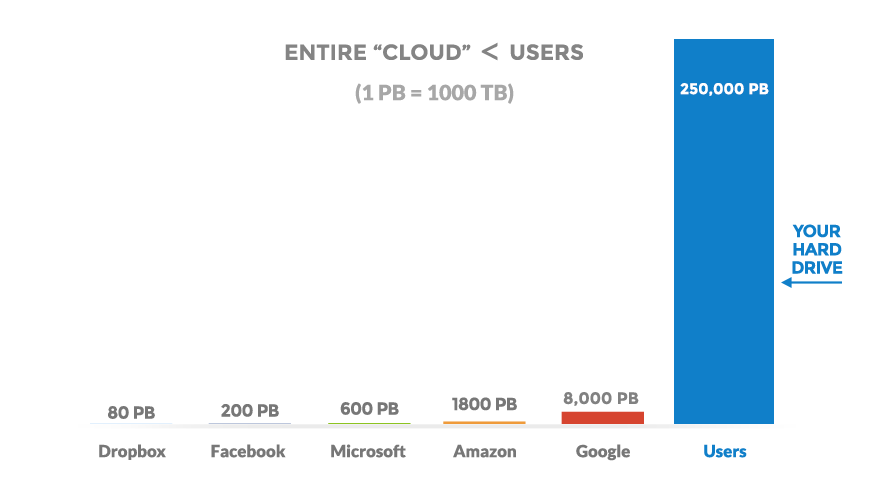
\includegraphics[width=\linewidth]{9}
\caption{Visualizing Cloud Storage vs. User Space }
\end{figure}

\subsection{Sybil Redundancy Attacks}
An attacker who would like to exploit the network by pretending that he/she has multiple redundant copies of a chunk, when he/she has only one, cannot do so, since each redundant copy is uniquely encrypted. Therefore, an attacker cannot pass heartbeats unless they have copies of the unique redundant copies. The client node should take steps to distribute its redundant copies to geographically distributed and independent nodes. If randomly distributed, the probability of the same redundant piece being hosted on the same controlled node is statistically quite small.  \\
%code formatting
%\begin{lstlisting}
%{
  %version: "0.1",
  %datetime: "1391212800",
  %filesize: "23124",
  %file_hash: "6e163442e29ec8d7538bc86fe2c4a48778e8ae2254632f0889da753b1c357b1b",
   %"uploads": [
  %{ "host_name":"mediafire" , "url":"http://www.mediafire.com/?qorncpzfe74s9"},
  %{ "host_name":"rapidshare" , "url":"http://rapidshare.com/files/130403982"}
 % ]
%}
%\end{lstlisting}

Even if the file is publicly shared, and the decryption key is known, the malicious actor cannot know the seed that was used to generate the heartbeats that it must respond to in order to receive payment. Furthermore, since the only information given about a chunk is its hash, an attacker can’t know which chunk is a redundant but unique copy of another. Therefore, due to random distribution and our standard methods of uniquely encrypting redundant copies, an attacker cannot execute a Sybil redundancy attack.   

\subsection{Cheating Client Node}
Let us imagine a scenario whereby a malicious actor would like to host file on the network, but avoid paying for said file, or intentionally rejecting correct heartbeats in order to avoid payment. In this case, there would be a disagreement between the two nodes, and the transaction would cease. Merkle roots embedded in the blockchain, as described previously, serve as sufficient and irrefutable proof of the validity of challenges from the client.

\subsection{Hostage Byte}
The hostage byte attack was first described by Vitalik Buterin, in which a malicious farmer transfers data to a client but holds the last piece of data “hostage” for a higher payment \cite{16}. We address this with our erasure encoding scheme, so that the chunks required to reassemble the file are not linear. As long as the client keeps the bounds of its erasure encoding a secret, the malicious farmer cannot know what the last byte is.   

\section{Outsourceable Heartbeats}
Traditional decentralized networks, such as Bitcoin, \cite{3} rely on consensus algorithms in order to function. They more directly use algorithms such as proof-of-work, \cite{3} in which computational power determines network consensus. Unfortunately, these mechanisms require for a majority of the nodes on the network to be honest. This has destroyed smaller cryptocurrencies such as Terracoin \cite{17} and many others, where the majority of the nodes did not behave honestly, known as a 51\% attack. Bitcoin itself has had problems itself with potential 51\% attacks \cite{18}.  Furthermore, these algorithms waste massive amounts of computational power in order to ensure security \cite{19}, although some advancements have been made in cryptocurrencies such as Peercoin \cite{19}.  \\

A 51\% attack on a standard cryptocurrency network like Bitcoin have little effect on a majority of the network. Only users transacting at the time of the attack could be defrauded, not the rest of the network. This is different for a data-based network as an attacker could alter the state of the chunks the network, and cause data loss. Depending on the data, that could have catastrophic effects on the network, and perhaps lead to the full failure of the network. In this way, we cannot rely on consensus alone to determine the state of the chunks stored on the network. \\

We instead designate the client as the ultimate decider in the network. After all, it is the client who is paying for the storage space on the network. We have previously established methods, such as embedding the Merkle root of the challenges in the blockchain, so although the client is the ultimate decider, the client cannot cheat the farmer. Using the heartbeat algorithm, it doesn’t matter how many dishonest or colluding nodes are on the network. Malicious nodes will not be able to pass challenges, and unique and encrypted redundant copies will ensure that colluding nodes and Sybil attacks are not possible. \\

The question remains of how to handle heartbeats when the client is offline. We cannot expect a traditional client to be online all of the time, so we must devise trustless methods in order to validate heartbeats and pay the farmers. We propose several methods that are individually and collectively valid methods of validation and payment. \\

\subsection{Client Controlled}
The easiest method is simply that the client has control and access to their own online hardware, say, for example, a simple VPS server that can be purchased for only a few dollars a month. To offset the cost, they could share it with other users or friends that they know. Operation is quite simple -- the server need only pass a challenge to a farmer periodically, and verify it against a predetermined response. This server could also handle the various payments to the farmers.

\subsection{Group of Verification Nodes}
Another method is to rely on groups of verification nodes (GVNs) that manage heartbeats and payment. A user will pass heartbeats and payments to a GVN. In an M-of-N multisig scheme, we use N of N, where N is the number of nodes in GVN. In this way, a single non-colluding and honest node is able to disprove and block payment for any colluding nodes. At the client’s discretion we may use M < N schemes. Sia \cite{20} describes some methods that could be used to eject colluding nodes. In order to keep the client as the ultimate decider, we additionally require that a transaction be crafted that returns funds to the client, but one which is not broadcasted, so that at any point and time the client can retrieve any unspent funds. We can further add proof-of-existence methods \cite{4} [5] \cite{7} so that all actions taken by these node groups are publicly auditable through a blockchain. 

\subsection{Buried Keys}
The heartbeat responses themselves could be the private or access keys to funds. After responding, the farmer could then redeem their keys for payment directly from the network or from a GVN. Alternately, a decentralized payment service managed by smart contracts could be a solution by itself or in concert with a GVN. 

\subsection{Dust and Anonymizing}
GVNs allow us to collate millions of verifications and payments into singular payments to the farmers. Ideally, the GVN and farmer would establish a micropayments channel, and the farmer would be paid via the GVN instantly per verification. In this way, we avoid making millions of small dust transactions. Furthermore, a GVN will provide anonymity to the users, as funds can be mixed within a GVN. Therefore, there is not a direct or indirect links between a user’s funds and their files.

\subsection{Extending GVNs}
As we lay out the ideas for Storj, there are several other methods being developed that could handle heartbeats and trustless payments. These include Notary Chains \cite{7}, oracles \cite{21}, smart contracts, Turing-complete blockchains \cite{22}, P2P networks, blockchains, quorums \cite{20}, and scratch-off puzzles \cite{23}. Each one of these methods could be a useful and trustless method of handling heartbeats and payments. While MetaDisk \cite{1} will serve as the first implementation of a node in a GVN, these other methods could also serve as nodes in a GVN. Our core goal is to have the client as the ultimate decider. The client can either handle these tasks, or have full power over which algorithms the client feels most comfortable with protecting the client’s data. 

%insert Figure 10
\begin{figure}[h!]
\centering
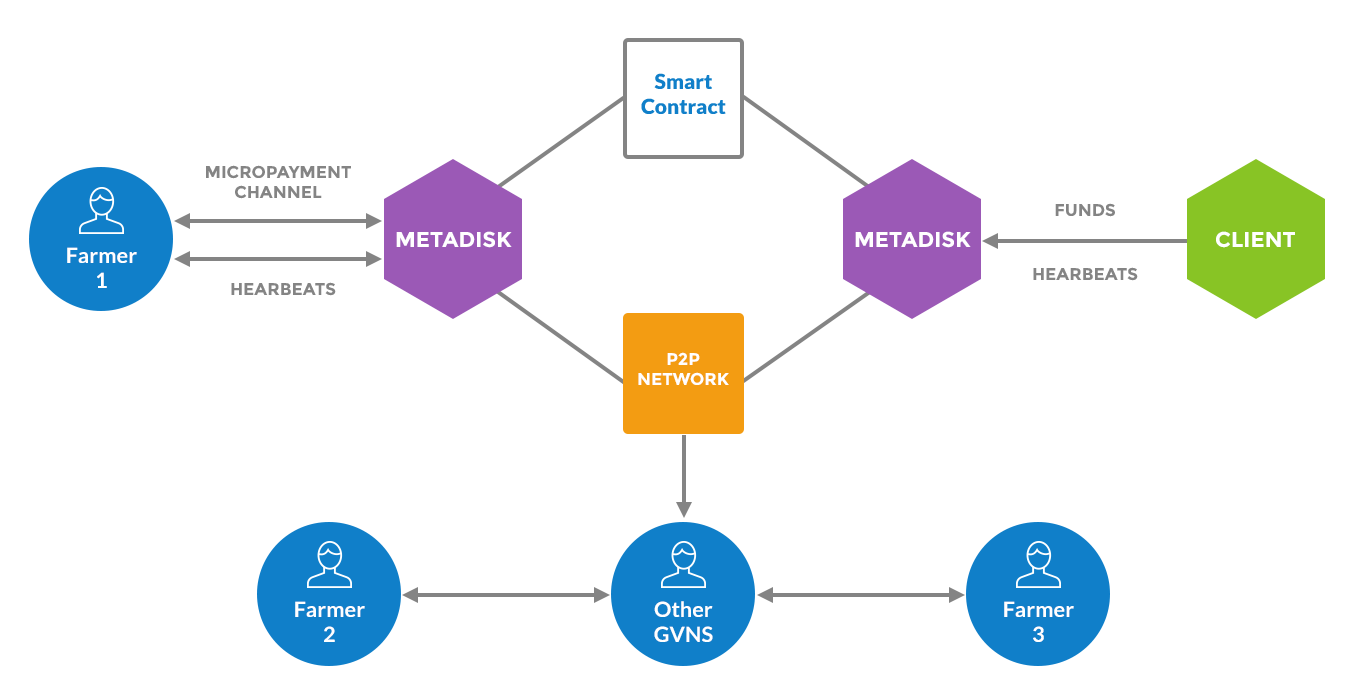
\includegraphics[width=\linewidth]{10}
\caption{Visualizing Cloud Storage vs. User Space }
\end{figure}

\section{Calculations}
Chance of failure of k-of-n erasure coding assuming probability p every chunk stays online:

{\centering
$\Pr_{failure}(n,k,p) = \displaystyle \sum_{i=0}^{k-1} p^{k}(1-p)^{n-k }{n \choose k}$
\\}


%code formatting
\begin{lstlisting}
n=9  k=3  p=0.5  : 0.08984375
n=9  k=3  p=0.75 : 0.0013427734375
n=9  k=3  p=0.9  : 2.998e-06
n=9  k=3  p=0.98 : 4.4481536e-11
n=9  k=2  p=0.5  : 0.01953125
n=9  k=2  p=0.75 : 0.000106811523438
n=9  k=2  p=0.9  : 8.2e-08
n=9  k=2  p=0.98 : 2.26304e-13
n=18 k=6  p=0.5  : 0.0481262207031
n=18 k=6  p=0.75 : 3.42457205988e-05
n=18 k=6  p=0.9  : 5.26615912e-10
n=18 k=6  p=0.98 : 6.39103033491e-19
n=18 k=4  p=0.5  : 0.00376892089844
n=18 k=4  p=0.75 : 3.41446138918e-07
n=18 k=4  p=0.9  : 6.0742e-13
n=18 k=4  p=0.98 : 2.52627700941e-23
n=36 k=12 p=0.5  : 0.0144083598279
n=36 k=12 p=0.75 : 2.6154613168e-08
n=36 k=12 p=0.9  : 1.97780182001e-17
n=36 k=12 p=0.98 : 1.62829264468e-34
n=36 k=8  p=0.5  : 0.000156275578775
n=36 k=8  p=0.75 : 4.18707347677e-12
n=36 k=8  p=0.9  : 4.09844839229e-23
n=36 k=8  p=0.98 : 3.90921460941e-43
n=72 k=24 p=0.5  : 0.00147138026506
n=72 k=24 p=0.75 : 1.93774114606e-14
n=72 k=24 p=0.9  : 3.6364801867e-32
n=72 k=24 p=0.98 : 1.39046479388e-65
n=72 k=16 p=0.5  : 3.26998411087e-07
n=72 k=16 p=0.75 : 8.13002111627e-22
n=72 k=16 p=0.9  : 2.44918555677e-43
n=72 k=16 p=0.98 : 1.2363767277e-82
\end{lstlisting}

%code formatting
Code:
\begin{lstlisting}
def fac(n): return 1 if n==0 else n * fac(n-1)
def choose(n,k): return fac(n) / fac(k) / fac(n-k) 
def prob(n,k,p): return choose(n,k) * p ** k * (1-p) ** (n-k)
def prob_fail(n,k,p): return sum([prob(n, i, p) for i in range(0, k)])
\end{lstlisting}
Therefore, with sufficient parameters for erasure encoding, in addition to recovery methods described in above, the statistical chance of chunk or file lost is quite small. 

\section{Conclusion}
We have outlined a peer-to-peer cloud storage network implementing end-to-end encryption which allows users to transfer and share data without reliance on a third party data provider. We have addressed problems such as Sybil attacks and peer disconnects by using uniquely encrypted redundant copies, and a heartbeat algorithm which periodically checks for file availability and integrity. By using cryptocurrency, we can provide the proper incentives for growth of the network and the trading of data between a client and farmer. We give the client full power over the algorithms that handle verification and payments for their files. Using these methods, we hand back control of cloud data to the users. 



\bibliographystyle{unsrt}
\begingroup
  \raggedright
  \bibliography{storj}
\endgroup


\end{document}
